\documentclass[10pt,a4paper]{article}
\usepackage[latin5]{inputenc}
\usepackage{amsmath}
\usepackage{cleveref}
\crefname{section}{§}{§§}
\usepackage[a4paper, margin=1.25in]{geometry}
\usepackage{amsfonts}
\usepackage{amssymb}
\usepackage{graphicx}
\usepackage[backend=biber]{biblatex}
\bibliography{Hackathon}
\author{csaaw}
\title{Title!}

\begin{document}
\maketitle

\section*{abstract}

\section{introduction}
\label{sec:intro}

This paper explores the question: how much can the chemical composition of pottery fragments tell us about the evolving connections between settlements in Bronze Age Greece? 




\section{literature review}
\label{sec:litrev}

In this section, two categories of literature are surveyed: (a) theories of Bronze Age trade relevant to the movement of ceramics, and (b) relevant archeometric and modeling methods.

Our dataset includes ceramic shreds from the 7th century BC to the Roman period, but mainly consists of works from the Late Helladic Period - III (LH III, see \cref{fig:timeline} for a chronology)
\cref{fig:seamap} is a map with dashed lines encoded hypotheses about prominent sea routes in the late Bronze Age.  


Maps like \cref{fig:seamap} are of tremendous historical significance if they can be constructed accurately. A common way to map trade is to identify artifacts that have been transported from their location of origin.  How do researchers infer where ceramic objects and shreds originate? 

\section{Motivation/Dataset}
\subsection{Motivation and Summary Stats}
Archaeological studies has been actively inviting the analytical methods from
the entire spectrum of social science studies. However, when it comes to the
application of machine-learning techniques, we have not seen much done recently.
Therefore, we set out to explore the archaeological databases, searching for
datasets that are rich enough, in terms of dimensions of the observables.

Baring the capability of machine-learning in mind, we found the 
Lawrence Berkeley National Laboratory (LBNL) Nuclear Archaeology Program
Archives %\cite?? [the archive]
of particular interest, as it not only contains geographical and historical
records of the artifacts, it also carry the chemical compositions for most of
its records.


Due to limited time and resources, we focused exclusively on the Greece records,
totaling 886 pieces of artifacts from ancient Greece, discovered from 31
archaeological sites\footnote{30 in Greece, and one (Perati in Attica) in
Turkey.}.  The time frame in our sample covers from the Early Helladic era
(around 3200 BC) to Roman Republic. 

\subsection{Data manipulation}
For the records of artifacts from Greece, the dataset came with 1,198
observations in the begining, pulled directly from \verb|http://core.tdar.org/|.
The variables include the discovery site, the associating era, geo-coordinates
and the chemical compositions of 33 elements\footnote{Elements are:
    \textit{Al Ca V Dy Mn Na K Sr As U Eu Ba Sm La Ti Lu Nd Co Sc Fe Ce Yb Cs Ta
    Sb Cr Th Ni Rb Tb Hf Zn}
}. However, the chemical composition
data is not complete. Thus, we dropped a subset of observations as well as
insignificant variables of elements (\textit{Sb Ba As Sr V}) to obtain a sample
of 886 observations. 




\section{Problem Formulation}
 


\section{Methdology}
\section{Methodology}

\label{sec:methodology}

%822,27,20

We are interested in analyzing artifacts from $N=20$ archaeological sites. We denote by $X^i$ the collection of artifacts in the $i$-th site, that is $X^i=\{x^i_1,x^i_2,\dots,x^i_{n_i}\}$, where $n_i$ is the number of artifacts in site $i$ and $x^i_m$ refers to the $m$-th artifact in the $i$-th site.

The chemical composition data available for each artifact consists of the concentration of $L=27$ different chemicals. Artifact $x^i_m$ then consists of the (normalized) vector containing these chemical concentrations.

The simplest way to compare the chemical composition of two artifacts is through their square distance

$$ \| x^i_m - x^j_l \|^2 = \sum_{k=1}^L ( (x^i_m)_k - (x^j_l)_k )^2$$

where $(x^i_m)_k$ refers to the $k$-th (normalized) chemical concentration of artifact $x^i_m$.

This distance is taken to represent reasonably when two artifacts are similar. If their distance is small they are considered more similar than if their distance is large. The square distance can serve as the basis to construct many other similarity measures, for instance

$$ k(x^i_m,x^j_l) = \exp(-h\|x^i_m - x^j_l \|^2)$$

where $h>0$ is a parameter. This corresponds to the widely used Gaussian kernel. Other similarity measures $k$ between artifacts based on their chemical composition are possible. The question of which similarity measure between artifacts based on chemical compositions is more appropriate for statistical inference is an important one, but we do not consider it further.

The challenge is to construct a similarity measure between different sites based on the similarities ${k(x^i_m,x^j_l)}$ between their respective artifacts. We propose constructing such similarity function by looking at the average similarity between all pair of artifacts $(x^i_m,x^j_l)$ belonging to sites $X^i$ and $X^j$, respectively, given by

$$S(X^i,X^j) = \frac{1}{n_i n_j} \sum_{m=1}^{n_i} \sum_{l=1}^{n_j} k(x^i_m,x^j_l).$$

There is a theoretical justification for this similarity measure between archaeological sites, given by the theory of kernel mean embedding. This theory will be described in Section~\ref{sec:kme}.

We now wish to illustrate how well the similarity measure $S$ performs in finding similarities between archaeological sites based on the chemical composition of their respective artifacts. We do this by providing a network plot of the archaeological sites, where two sites $X^i$ and $X^j$ are considered connected if their similarity $S(X^i,X^j)$ is larger than a prescribed threshold. The results are illustrated in the figures~\ref{fig:whatevs}.

\section{Similarity}

\label{sec:similarity}

In this section we detail the way in which similarities are computed. We draw inspiration from a well known set of methods in the machine learning community, and acknowledge that the mathematical machinery might not be familiar to the intended audience. Therefore the reader is invited to skip this section on the first read and come back to it when necessary.

We think of the chemical composition vectors $\{x^i_m\}_{m=1}^{n_i}$ corresponding to the artifacts in the $i$-th site $X^i$ as consisting of instances from some distribution $P_i$.

...

\subsection{Reproducing Kernels}

\label{kernels}

To build a network we need an appropriate notation of similarity between sites (probability densities). We desire the probability densities to inhabit a well behaved space of functions (a Hilbert Space) where a common notion of similarity exists. We propose to embed each probability density into the so called RKHS of a kernel $K$ and use the inner product in this space as the similarity measure.

The similarities we propose capture similarities among probability densities as elements of a function space. To determine these similarities we need first determine the function space the probability densities inhabit. The function space we will use is the so called Reproducing Kernel Hilbert Space (RKHS) associated to a reproducing kernel. We now define these mathematical objects.

A {\it reproducing kernel} is a symmetric function $k: \sx\times \sx\rightarrow \mathbb{R}$ for which there exists a unique Hilbert space of functions $\sh$ such that $k(\cdot,x)\in \sh$ for all $x\in \sx$ and the reproducing property

\begin{align}

f(x) = \left<f,k(\cdot,x)\right>

\end{align}

holds for all $f\in\sh$ and all $x\in \sx$

\subsection{Kernel Mean Embedding}

\label{kme}

Let $k$ be a reproducing kernel as in section, the {\it kernel mean embedding} of the probability density $P$ in the RKHS $H$ of $k$ is

$$\phi_0(P) = \int k(\cdot,x)P(x) dx$$

Since the true form of $P$ is unknown we use the available data to estimate the KME. Let ${x_l}_{l=1}^n$ be an iid sample from $P$, then the empirical kme of $O$ is

$$\phi(P)=\frac{1}{n}\sum_{l=1}^n k(\cdot,x_l).$$

Although $\phi(P)$ depends on the sample we will omit this dependencies to simplify notation.

With this tool at hand, we define the similarity between site $i$ and site $j$ as the inner product of their corresponding KME's.

\begin{align*}

S(X^i,X^j)&=\langle \phi(P_i),\phi(P_j) \rangle_H \\

&= \frac{1}{n_i n_j} \sum_{l=1}^{n_j} \sum_{m=1}^{n_j} \langle k(\cdot,X_l^i),k(\cdot,x_m^j) \rangle_H \\

&= \frac{1}{n_i n_j} \sum_{l,m} k(x^i_l,x^j_m)

\end{align*}

where the last equality follows from the reproducing property.


\section{Results/explanations}
  
As explained in the dataset section, we divide the dataset into different eras and analysed the data using proposed method. One can see in \ref{fig:Overall_network} the evolution of the network between different sites. Mycenae wasn't the prominant center until 1300BC. The city is networked to may places as time evolves. Berbati became the prominant city after 1000 bc (?? citation), which can be seen from the network.
We also combine the data from all the eras and see how different sites are connected. 


\begin{figure}
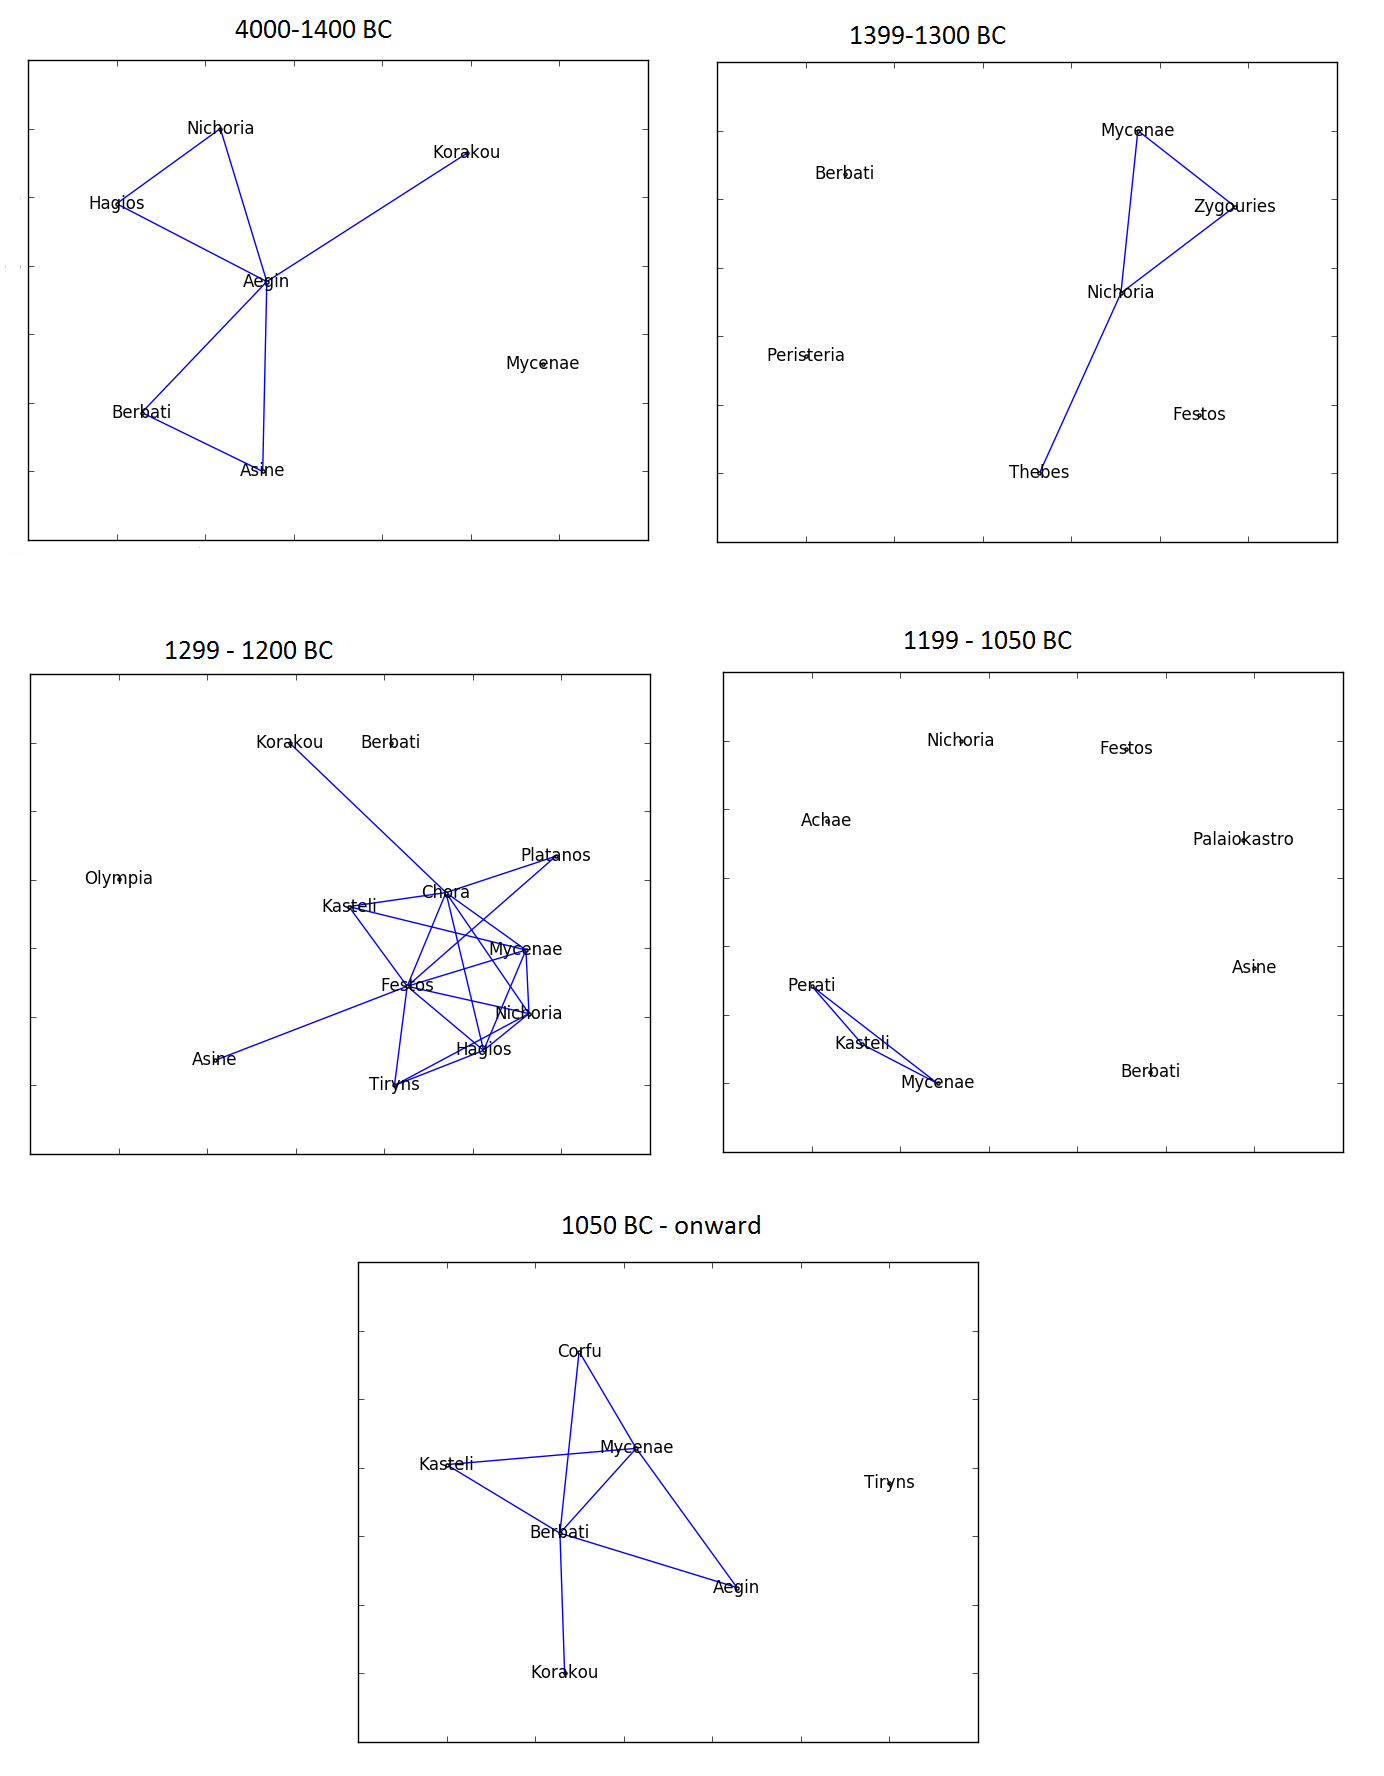
\includegraphics[width=\textwidth]{Network_evolution.png}
\caption{Evolution of networks of the Archaeological sites}
\end{figure}


\begin{figure}
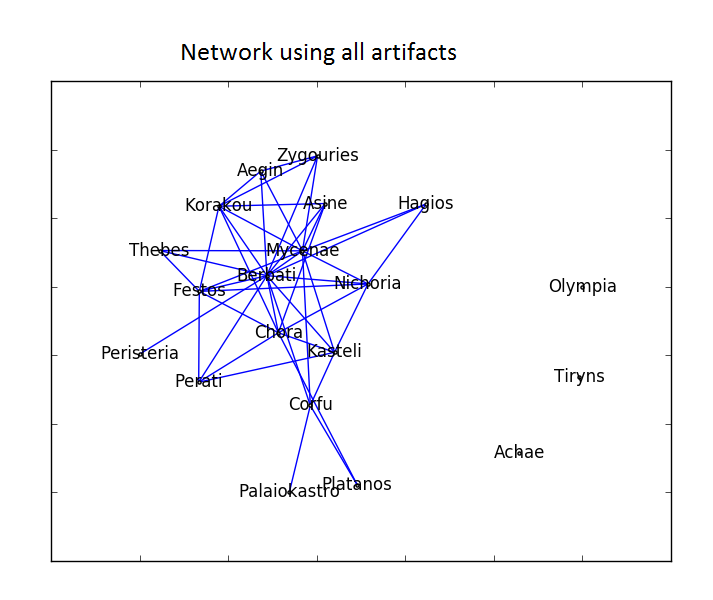
\includegraphics[width=\textwidth]{Overall_Network.png}
\caption{Overall network of the Archaeological sites}
\end{figure}

\section{Conclusion}
 


\newcommand{\foo}{\hspace{-2.3pt}$\bullet$ \hspace{5pt}}
\begin{figure}
\scalebox{1}{
\begin{tabular}{r |@{\foo} l}
 7000 & Beginning of widespread use of pottery in Mediterranean.
Aegina as maritime center\\
3200-2000 & Early Helladic  \\
3200-2500 &  High point of Anatolian trade network \\
2000-2200 & Disruption of trade between Cyclades, Mainland, and Crete. Upheaval in Mainland \\
2000-1550 & Middle Helladic. Protopalatial and Neopalatial buildings in Crete \\
1650-1500 & Late Helladic I / Late Cycladic I / Late Minoan IA \\
1500-1400 & Late Helladic II \\
1400-1300 & Late Helladic III A \\
1300-1200 & Late Helladic III B. High point of Mycenaean influence on trade\\
1200-1050 & Late Helladic III C \\
1050- & End of Bronze Age. Transitional Period: Argos, Asine and Berbati rise to prominence. 

\end{tabular}
}

\caption{Timeline of Events of Interest (all dates B.C.)}

\label{fig:timeline}
\end{figure}

Qualitative methods include categorization by geometric features, and material features. For instance, Davis\cite{davis1979late} classifies pieces from LH I Korakou by shapes, as well as surface and burnishing, measured by the eye against a color chart.  The task is to sort shreds and pieces by style, and also material - these two elements are necessary to differentiate cases where a style travels but pieces are built from local materials. A qualitative study we'll discuss in detail later is that of Rutter\cite{rutter1975ceramic} - he uses the shapes and visible properties of pottery found in Korakou to argue that those pieces were erroneously categorized as Mycenaean. That is: qualitative differences are used to prove a classification claim.  


\begin{figure}
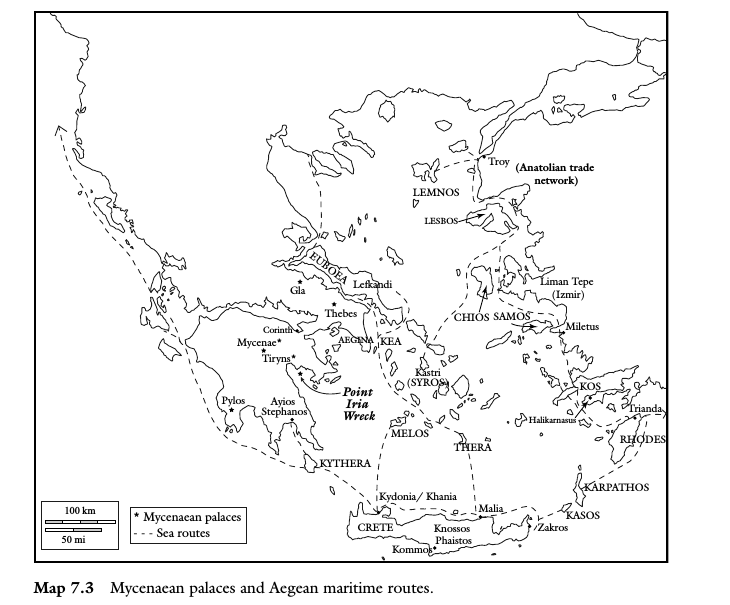
\includegraphics[width=\textwidth]{pottery2.png}
\caption{image from \cite{demand2011mediterranean}}
\label{fig:seamap}
\end{figure}

Quantitative work in classifying pottery mainly uses data from neutron activation analysis or spectral analysis of paints.  This paper uses a neutron activation analysis dataset from the LBNL archeometry archives. The extant work on this dataset (which contains subsections for many geographical areas across the world) has mostly been conducted by Mommsen and colleagues. This work has two main goals: first, to be a proof of concept for quantitative analysis by reproducing known results from limited data, and second, to discover previously unknown connections as a bridge for further inquiry, both qualitative and quantitative.  So for instance, in \cite{mommsen2002complete}, Mommsen et al take their model to succeed by matching existing predictions about early recipe variation in Argolid pottery suggested by Hoffman et al, and by adding new predictions in the case of suggesting a pattern of export from Chania to Cyprus of cream ware.  Grave  et al\cite{grave2014ceramics} follow a similar method of combining the LBNL dataset with other information, also with Cyprus late Helladic wares. 


\begin{figure}
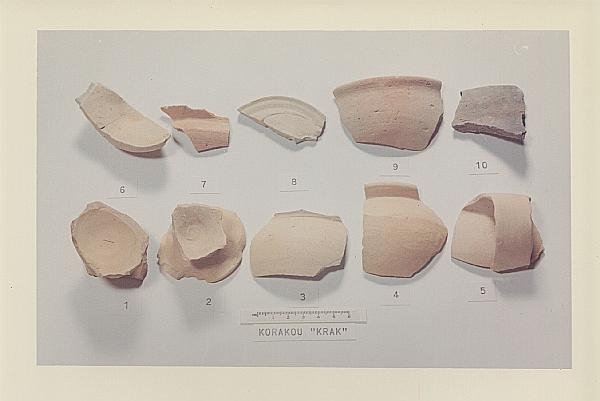
\includegraphics[width=\textwidth]{korakou}
\caption{Example of shreds in the database}
\label{fig:sample}
\end{figure}





\section{method}

\printbibliography

\end{document}
